\documentclass{llncs}

\usepackage[utf8]{inputenc}
\usepackage{tikz}

\usepackage{algorithm}
\usepackage{algorithmic}
\usepackage{amsmath}
\usepackage{diagbox}
\floatname{algorithm}{Algoritmo}
\renewcommand{\listalgorithmname}{Lista de algoritmos}
\renewcommand{\algorithmicrequire}{\textbf{Entrada:}}
\renewcommand{\algorithmicensure}{\textbf{Salida:}}
\renewcommand{\algorithmicend}{\textbf{fin}}
\renewcommand{\algorithmicif}{\textbf{si}}
\renewcommand{\algorithmicthen}{\textbf{entonces}}
\renewcommand{\algorithmicelse}{\textbf{si no}}
\renewcommand{\algorithmicelsif}{\algorithmicelse,\ \algorithmicif}
\renewcommand{\algorithmicendif}{\algorithmicend\ \algorithmicif}
\renewcommand{\algorithmicfor}{\textbf{para}}
\renewcommand{\algorithmicforall}{\textbf{para todo}}
\renewcommand{\algorithmicdo}{\textbf{hacer}}
\renewcommand{\algorithmicendfor}{\algorithmicend\ \algorithmicfor}
\renewcommand{\algorithmicwhile}{\textbf{mientras}}
\renewcommand{\algorithmicendwhile}{\algorithmicend\ \algorithmicwhile}
\renewcommand{\algorithmicloop}{\textbf{repetir}}
\renewcommand{\algorithmicendloop}{\algorithmicend\ \algorithmicloop}
\renewcommand{\algorithmicrepeat}{\textbf{repetir}}
\renewcommand{\algorithmicuntil}{\textbf{hasta que}}
\renewcommand{\algorithmicprint}{\textbf{imprimir}} 
\renewcommand{\algorithmicreturn}{\textbf{devolver}} 
\renewcommand{\algorithmictrue}{\textbf{cierto }} 
\renewcommand{\algorithmicfalse}{\textbf{falso }} 


\pagestyle{plain}

\title{Implementación de un Algoritmo Inmune Artificial basado en Selección Clonal para resolver el UTRP}
\author{Cristopher Arenas\\\texttt{cristopher.arenas@alumnos.usm.cl}}
\institute{Departamento de Informática\\Universidad Técnica Federico Santa María}

\renewcommand{\tablename}{Tab. }

\begin{document}
\maketitle

\begin{abstract}
Los algoritmos inmunes artificiales (AIA) son estrategias de resolución de problemas evolutivos, lo que quiere decir que cambian con el tiempo y representan analogías de ciertos comportamientos biológicos. Estos algoritmos se puede utilizar en ciertos problemas, como por ejemplo el Urban Transit Routing Problem UTRP, en el cual se pretende encontrar rutas que satisfagan a operadores de los buses y a las personas que transportan. Por medio de un modelamiento, una representación del problema y la resolución por medio de un AIA se encontrará una solución que pueda satisfacer un conjunto de restricciones y trabajar con ciertos objetivos.
\end{abstract}

\section{Introducción}

El diseño de un sistema de transporte que sea eficaz y eficiente es un problema importante en la actualidad y es de gran relevancia en las grandes urbes. porque implican translados de muchas personas en todo momento del día. Existen varios problemas asociados al diseño un buen sistema de transporte, los cuales se enfocan principalemente en establecer una buena planificación de horarios para conductores o buses, o definir enrutamientos que beneficien tanto a los usuarios como a las empresas operadoras de buses. El Urban Transit Routing Problem o UTRP \cite{metaheuristic2010} consiste en definir enrutamientos para una red de transporte público que sean capaces de reducir costos temporales tanto para pasajeros, como para operadores de buses. Es así como el UTRP se plantea como un problema multi-objetivo que requiere de técnicas que se encarguen de minimizar ambos costos.\\

En la literatura \cite{NewHaEOps,john2014improved} se han propuesto varios algoritmos, principalmente evolutivos, que tienen inspiración en fenómenos biológicos, para obtener soluciones en el UTRP. Los algoritmos propuestos establecen la evolución de soluciones iniciales definidas mediante estratégias o heurísticas, las cuales son modificadas mediante operadores de transformación, de manera de encontrar en pequeñas vecindades soluciones similares que puedan ser más beneficiosas para pasajeros u operadores de buses. Los Algoritmos Inmunes Artificiales o AIA \cite{introduction,sia} corresponden a una familia de algoritmos que se basan en el sistema inmune de un organismo, donde un conjunto de anticuerpos debe enfrentarse a un virus o infección. Los anticuerpos funcionan por medio de procesos adaptativos, pues una vez que encuentran la mejor forma de curar una enfermedad, se capacitan para tomar acción ante futuras infecciones.\\

En el presente trabajo considera una propuesta de AIA, con sus respectivos procesos de transformación y selección. Esto es, mediante la definición de operadores de transformación específicos para el UTRP y por medio de la presentación de parámetros relevantes para los procesos de selección. En el capítulo 2 se presentará el estado del arte del UTRP y se mostrarán enfoques y técnicas utilizadas para encontrar soluciones. El capítulo 3 describe en detalle el UTRP, mencionando las variables, parámetros y restricciones que considera el problema, asi como los objetivos que deben minimizarse. El capítulo 4 muestra la representación de elementos importantes para el problema. Los capítulos 5, 6, 7 y 8 presentan el AIA propuesto, detallando los pasos necesarios para generar soluciones factibles, parámetros asociados, operadores de tranformación y otras consideraciones importantes. El capítulo 9 detalla una serie de experimentos que se realizarán sobre instancias utilizadas en la literatura, cuyos resultados obtenidos se mostrarán en el capítulo 10.


\section{Estado del Arte}
El problema de enrutamiento de tr\'ansito urbano (UTRP por sus siglas en ingl\'es) involucra la ideaci\'on de rutas para el transporte p\'ublico.
Se trata de un problema NP-Duro altamente complejo, y resolverlo involucra invariablemente un ciclo de
generaci\'on y prueba de grupos de rutas candidatas. La mayor parte de literatura lo considera parte de un problema de escala mayor, el Urban Transit Network Design Problem (UTNDP por sus siglas),
el cual es dividido tanto en el UTRP como UTSP (Urban Transit Scheduling Problem), y tal como se puede diferir de sus nombres, el UTSP
tiene un enfoque de agendar los tiempos de llegada de los medios de transporte, mientras que el UTRP se enfoca en las rutas que estos
utilizan, ambos para mejorar el sistema de transporte urbano en las ciudades.\\
Los primeros acercamientos al UTRP lo tratan como un problema mono-objetivo. En~\cite{metaheuristic2010} se
comparan dos acercamientos de b\'usqueda local para resolver el problema. En este
caso se consideran dos objetivos: la distancia acumulada de todos los pasajeros
del bus y el n\'umero de trasbordos para la demanda completa. Se considera toda la demanda como satisfecha y el tiempo
promedio que cada usuario destina en viajar es
el menor posible. Adem\'as, se considera que cada ruta del conjunto est\'a libre de ciclos y retrocesos;
el conjunto de rutas est\'a conectado; hay exactamente $r$ rutas en el conjunto y el n\'umero de nodos en cada
ruta debe ser mayor a uno y no debe exceder el valor m\'aximo definido. \\
La funci\'on objetivo est\'a dada por la suma ponderada de ambos objetivos.
La inicializaci\'on se realiza de manera aleatoria respetando el largo establecido. Se
utiliza el movimiento \emph{Make-small-change}, que considera 3 posibilidades: Agregar un nodo en
la \'ultima posici\'on de la ruta, borrar el primer nodo de la ruta e invertir el orden de nodos en la ruta.
En~\cite{memetic2011} se propone un algoritmo mem\'etico cuyo objetivo es minimizar la suma del costo
para los usuarios y la demanda insatisfecha para la red de rutas. La inicializaci\'on se reliza
de manera aleatoria, se utiliza cruzamiento de rutas en un punto y mutaci\'on de una ruta por otra ruta factible. Para
la b\'usqueda local se seleccionan uno o dos cromosomas aletatoriamente, y se combinan de acuerdo a: (1) 
movimiento 2-opt, (2) intercambio de dos paraderos y (3) reubicaci\'on de una parada. Al final del proceso
se seleccionan los mejores $\mu$ cromosomas padre y $\lambda$ cromosomas hijo.
En~\cite{jiang2010improved} se utilizan colonias de hormigas para el UTRP. A diferencia de otros problemas resueltos con colonias de
hormigas, las hormigas no deben recorrer todos los nodos, sino que deben ir desde cierto nodo hasta otro.
Se toma como consideraci\'on que cada nodo podr\'a tener a lo m\'as 4 vecinos y las conexiones con estos ser\'an aquellas pertenceciente a
un conjunto de arcos permitidos. Si en alg\'un momento la ruta escogida por la hormiga no cumple
alguna de las restricciones (por ejemplo, ciclos en el recorrido), la hormiga se declara muerta y se castiga el
camino escogido.\\

Es posible encontrar acercamientos multi-objetivo para otros problemas similimares. Josefowiez, Semet y Talbi
en~\cite{vrprb} utilizan diversificaci\'on elitista y modelo de islas para el vehicle routing problem con
dos objetivos: minimizaci\'on del largo de las rutas y la diferencia entre el tama\~no de la ruta m\'as larga y la m\'as corta.
En este caso se utiliza ranking de dominancia para evaluar a los invididuos, donde los individuos no dominados de la poblaci\'on
forman el conjunto $E_1$ de ranking 1 y el resto de los individuos se agrupan en conjuntos $E_k$ donde cada elemento es dominado
por todos los elementos de los conjuntos anteriores.
En~\cite{ttvrp} se propone un MOEA h\'ibrido que incorpora b\'usqueda local y el concepto de optimalidad de Pareto para el
problema de encontrar una programaci\'on de rutas que cumpla con todas las entregas de una empresa de despacho, minimizando las distancias
recorridas y el n\'umero de camiones. Al igual que en el caso anterior se utiliza un ranking de fitness de Pareto para evaluar la calidad
de las soluciones. Zhang, Wang y Tang~\cite{events} investigan el problema de dise\~no de rutas para mega-eventos donde hay un gran
tr\'afico de transporte p\'ublico y se requieren rutas adicionales para el transporte de las personas que participan de un evento,
a su lugar de destino. En~\cite{events} se utiliza un algoritmo gen\'etico cuya funci\'on de evaluaci\'on es la distancia total del
conjunto de rutas. Adem\'as, se utilizan dos penalizaciones: la primera se aplica por cada nodo de destino que qued\'o fuera de ruta y
la segunda se aplica si la distancia total de una ruta supera la m\'axima distancia permitida.\\

Acercamientos multi-objetivos espec\'ificos para el UTRP se pueden encontrar en~\cite{zhang2010multi} donde se utiliza un algoritmo
evolutivo que usa el operador \emph{Make-small-change}. En este caso se utiliza el concepto de dominancia de Pareto para construir
el conjunto de soluciones. Este algoritmo entrega buen conjunto de rutas desde el punto de vista de los pasajeros y con mejores costos
para operadores en comparaci\'on a un algoritmo mono-objetivo similar con el que se compar\'o. Mumford en~\cite{NewHaEOps} utiliza exactamente
el mismo modelado, pero agrega un operador de cruzamiento al algoritmo evolutivo. El operador de cruzamiento selecciona intercaladamente
rutas de ambos padres de manera tal de tener una cantidad equitativa de rutas de cada padre en el hijo. Posteriormente, en \cite{john2014improved} John, Mumford y Lewis presentan un acercamiento multi-objetivo mejorado basado en NSGAII, junto con los operadores de cruzamiento de \cite{NewHaEOps} y ocho operadores de mutación. En~\cite{GAUTRP}
se considera el mismo modelo y funci\'on objetivo que los anteriores, pero 
se realizan diferentes operaciones sobre un set de rutas para tratar de mejorar su calidad. Entre las modificaciones
se encuentran: una selecci\'on mediante ruleta de las rutas a modificar, una operaci\'on crossover entre dos rutas padres,
y la revisi\'on de factibilidad de los hijos, para finalmnente realizar una operaci\'on de mutaci\'on sobre dos rutas pertenecientes
al mismo set, intercambiando nodos aleatorios.\\

Para hacerse una idea de la complejidad real del problema es posible mencionar que el sistema de transportes de la ciudad de Santiago, Chile,
Transantiago cuenta con $372$ recorridos, y $11272$ paradas disponibles. Dichas paradas se distribuyen en siete unidades agrupadas por
zonas~\cite{datosGob}. Adem\'as, cuenta con 7 tipos de servicios entre los que se cuentan: servicios normales, cortos, expresos, variantes,
nocturnos, especiales e inyectados que operan en distintas condiciones horarias y de capacidad. Los estudios realizados en el caso
particular de Santiago coonsideran microsimulaciones de focos de congesti\'on considerando
diferentes escenarios de aumento de la capacidad vial, reversibilidad de las pistas y simulaci\'on de incidentes~\cite{alarcon2010}, 
mientras que en~\cite{cortes2009} se presenta un metodo de resoluci\'on para el problema de asignaci\'on de horarios, rutas y asignaci\'on
de choferes para una de las siete empresas del Transantiago (STP Santiago) que cuenta con aproximadamente 300 buses.
El autor aborda el problema mediante MIP (Programaci\'on Entera Mixta).

\section{Descripción del problema}

El problema considera inicialmente que se cuenta con algunas variables, tales como un grafo $G$; el cual representa una red de paraderos, lo que se puede entender, por ejemplo, como la estructura que se tiene en una ciudad. Cada vértice corresponde a un paradero, mientras que los arcos corresponden a las conexiones o caminos existentes entre dichos paraderos. Se considera que el grafo es no dirigido, lo que quiere decir que un arco entre dos vértices indica que hay una conexión en ambos sentidos entre los arcos que conecta. Las posiciones de cada vértice también son conocidas. Además, este grafo posee matrices simétricas, que poseen valores de tiempo de viaje entre paradas, demandas asociadas para cada vértice.

Como restricciones del problema se puede considerar lo siguiente \cite{NewHaEOps}:
\begin{itemize}
\item Cada ruta del conjunto de rutas está libre de ciclos y retrocesos.
\item El conjunto de rutas está conectado.
\item Hay exactamente $r$ rutas en el conjunto de rutas.
\item El número de nodos en cada ruta debe ser mayor a uno y no debe exceder el valor máximo definido.
\end{itemize} 

Con esto se asume que se sabe la cantidad de rutas tendrá el conjunto de rutas resultante, además de que tendrán un rango paraderos permitidos, los cuales están acotados por un valor mínimo y un valor máximo.

El UTRP consiste en satisfacer tanto a operadores de buses, como a los pasajeros que los utilizan. Es por esto que se tienen las siguientes funciones objetivo, dadas por las Ecuaciones \eqref{eq:fo1} y \eqref{eq:fo2} \cite{NewHaEOps}.

La Ecuación \eqref{eq:fo1} considera una minimización de los costos para el operador de buses. $d_{ij}$ representa la demanda  entre las paradas $i$ y $j$ y $\alpha_{ij}$ corresponde al camino más corto entre las dos paradas.

\begin{equation}
\label{eq:fo1}
min\mbox{ }\frac{\sum^n_{i,j=1}d_{ij}\alpha_{ij}(R)}{\sum_{i,j=1}^{n}d_{ij}}
\end{equation} 

Por otra parte, en la Ecuación \eqref{eq:fo2} se considera una minimización de los costos para los pasajeros. $t_{ij}$ corresponde al tiempo de viaje entre las paradas $i$ y $j$. 

\begin{equation}
\label{eq:fo2}
min\mbox{ }\sum^r_{a=1}\sum_{(i,j) \in r} t_{i,j} (a)
\end{equation} 

Al considerar el UTRP como problema multiobjetivo, se plantea una minimización de costos tanto para operadores de buses, con la demanda de pasajeros; como para pasajeros al considerar los tiempos de viaje.

\section{Representación}

Dentro del contexto del UTRP, se pretende determinar un conjunto de rutas a partir de distintos paraderos de buses preestablecidos, los cuales deben presentar un beneficio para los pasajeros y para el operador del bus.\\

Para las paradas se utiliza un grafo no dirigido, cuyos vértices corresponden a las paradas y los arcos a un camino entre las paradas. Un ejemplo de esta representación es la red de Mandl, la cual puede apreciarse en la Figura \ref{fig:mandl}.

\begin{figure}[!htb]
\begin{center}
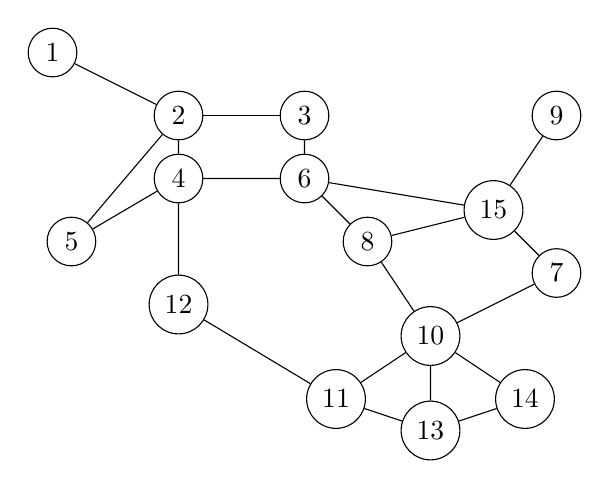
\begin{tikzpicture}[scale=0.8]
\node[draw,circle](1) at (0,0) { 1};
\node[draw,circle](2) at (2,-1) { 2};
\node[draw,circle](3) at (4,-1) { 3};
\node[draw,circle](4) at (2,-2) { 4};
\node[draw,circle](5) at (0.3,-3) { 5};
\node[draw,circle](6) at (4,-2) { 6};
\node[draw,circle](7) at (8,-3.5) { 7};
\node[draw,circle](8) at (5,-3) { 8};
\node[draw,circle](9) at (8,-1) { 9};
\node[draw,circle](10) at (6,-4.5) {10};
\node[draw,circle](11) at (4.5,-5.5) {11};
\node[draw,circle](12) at (2,-4) {12};
\node[draw,circle](13) at (6,-6) {13};
\node[draw,circle](14) at (7.5,-5.5) {14};
\node[draw,circle](15) at (7,-2.5) {15};

\draw (1) -- (2);
\draw (2) -- (3);
\draw (2) -- (4);
\draw (2) -- (5);
\draw (3) -- (6);
\draw (4) -- (5);
\draw (4) -- (6);
\draw (4) -- (12);
\draw (6) -- (8);
\draw (6) -- (15);
\draw (7) -- (15);
\draw (7) -- (10);
\draw (8) -- (10);
\draw (8) -- (15);
\draw (9) -- (15);
\draw (10) -- (11);
\draw (10) -- (13);
\draw (10) -- (14);
\draw (11) -- (12);
\draw (11) -- (13);
\draw (13) -- (14);
\end{tikzpicture}
\caption{Red de Mandl}
\label{fig:mandl}
\end{center}
\end{figure}

La representación escogida para manejar el UTRP es mediante un arreglo bi-dimensional que representa un conjunto de rutas. Cada fila será una ruta, la cual contiene un identificador asociado al número de ruta y posteriormente identificadores para los paraderos de buses. Estos paraderos se encuentran representados por una matriz de demandas, una matriz de tiempos de viaje y por un sistema de coordenadas (este último para modelar la posición de cada paradero).

En la Figura \ref{fig:repr1} se muestra un ejemplo de una representación de rutas el cual se pudo obtener a partir de la literatura existente sobre el UTRP \cite{metaheuristic2010}.

\begin{figure}[!htb]
\begin{center}
\begin{tabular}{|p{0.8cm}|p{0.8cm}|p{0.8cm}|p{0.8cm}|p{0.8cm}|}
\hline
R1 & 0 & 1 & 4 & 7\\
\hline
R2 & 0 & 3 & 6 & $*$\\
\hline
R3 & 1 & 2 & 5 & $*$\\
\hline
\end{tabular}
\caption{Representación para las rutas.}
\label{fig:repr1}
\end{center}
\end{figure}

Las matrices de tiempos de viaje y de demandas se representan mediante arreglos bidimensionales, donde la fila $i$ y columna $j$ aporta información entre el paradero $i$ y el paradero $j$.\\

Las soluciones para el algoritmo inmune artificial propuesto están dadas por un conjunto de rutas que siguen la estructura de la Figura \ref{fig:repr1}.

\section{Estructura del algoritmo}

El Algoritmo Inmune Artificial implementado está basado en un algoritmo de selección clonal genérico, propuesto por de Castro y Von Zuben \cite{read2012introduction}.

En el Algoritmo \ref{alg:aia} se muestran un pseudocódigo del algoritmo implementado. Un anticuerpo se entiende dentro del contexto de los algoritmos inmunes artificiales como una solución candidata. 

\begin{algorithm}
\caption{Algoritmo Inmune Artificial basado en Selección Clonal}\label{alg:aia}
\begin{algorithmic}[1]
\REQUIRE  Información del problema, información de instancia
\ENSURE Un conjunto de memoria $M$
\STATE Inicializar aleatoriamente población $P$ de tamaño \popsize
\STATE $g \leftarrow 1$
\WHILE{$g<=$\generaciones}
	\FOR{\textbf{cada} $p$ perteneciente a la población $P$}
		\STATE Calcular aptitud de $p$
	\ENDFOR
	\STATE Eliminar de la población $P$ anticuerpos dominados
	\STATE Seleccionar $mp$ de los mejores anticuerpos de $P$
	\STATE Generar un conjunto de clones $C$ de tamaño \clonsize{} con anticuerpos $mp$
	\FOR{\textbf{cada} clon $c$ perteneciente al conjunto $C$}
		\STATE $k \leftarrow$ numero de mutaciones a realizar de acuerdo a aptitud de $c$		
		\STATE Mutar $k$ veces el clon $c$
	\ENDFOR
	\STATE Copiar hasta $mp$ clones a la población $P$, basándose en ranking de pareto
	\STATE Seleccionar $mm$ anticuerpos de $P$
	\STATE Copiar los anticuerpos $mm$ al conjunto de memoria $M$
	\STATE Reemplazar $pp$ anticuerpos con anticuerpos generados aleatoriamente
	\STATE $g \leftarrow g+1$
\ENDWHILE
\end{algorithmic}
\end{algorithm}

\section{Parámetros del algoritmo}

El algoritmo considera los siguientes parámetros:

\begin{itemize}
\item \texttt{GENERACIONES}: criterio de término para el algoritmo inmune. Es la cantidad de iteraciones que deben ocurrir para que finalice el algoritmo. Posee valores de 0 a infinito.
\item \texttt{ALPHA} y \texttt{BETA}: representan variables de peso para ponderar las dos funciones objetivo y determinar una aptitud para una solución candidata. Posee valores entre cero y uno. La suma de ambas debe ser uno.
\item \texttt{POP\_SIZE}: representa el tamaño de la población $P$ en cada generación. Una generación está compuesta por un conjunto de soluciones candidatas factibles. Posee valores de 1 a infinito.
\item \texttt{CLON\_SIZE}: es el tamaño de la población de clones $C$ que se generarán en cada generación a partir de las mejores soluciones candidatas. Posee valores de 1 a infinito.
\item \texttt{PORCENTAJE\_MEJORES}: Porcentaje de mejores soluciones de la población que serán seleccionadas para mutarse en cada generación. Posee valores entre 0 y 1.
\item \texttt{PORCENTAJE\_CLONES}: porcentaje de mejores clones mutados que serán almacenados en el conjunto de memoria $M$. Posee valores entre 0 y 1.
\item \texttt{PORCENTAJE\_REEMPLAZO}: porcentaje de peores soluciones de la población que serán reemplazadas por soluciones aleatorias. Posee valores entre 0 y 1.
\end{itemize}

\section{Inicialización}

El conjunto de soluciones iniciales es generado aleatoriamente. Una solución está compuesta por $r$ rutas, donde cada está acotada por un mínimo y máximo de paraderos. El algoritmo \ref{alg:inicializacion} muestra los pasos de la generación de la población inicial.

Como fue mencionado en la representación del problema, una solución se compone por un conjunto de rutas. A su vez cada ruta se compone de un conjunto de paraderos. Para la generación de soluciones se debe iniciar con la asignación de paraderos, los cuales al agruparse constituyen una ruta. Finalmente, un conjunto de rutas genera una solución. 

Una ruta es generada escogiendo aleatoriamente la cantidad $q$ de paraderos que tendrá (acotada por el mínimo y máximo de paraderos). Después se selecciona aleatoriamente un paradero. Luego, se buscan los vecinos del paradero y se escoge aleatoriamente uno de ellos. Este proceso se repite hasta completar la cantidad $q$. Progresivamente, nuevas rutas son generadas de la misma forma, hasta completar $r$ rutas. Un conjunto de soluciones se generará repitiendo los pasos anteriores de rutas y paraderos hasta llenar la población $P$ con \popsize individuos.

Las soluciones que se generan en este algoritmo siempre son factibles, ya que satisfacen las cuatro restricciones del problema:
\begin{itemize}
\item Cada ruta del conjunto de rutas está libre de ciclos y retrocesos: el conjunto de vecinos a considerar no contiene paraderos que ya estén en la ruta.
\item El conjunto de rutas está conectado: es satisfecho considerando el conjunto de vecinos seleccionando solo aquellos paraderos con conexión directa, dado por el grafo de la red de paraderos. Si existe adyacencia entre dos vértices (paraderos) entonces se considera como un vecino.
\item Hay exactamente $r$ rutas en el conjunto de rutas: al generar solciones iniciales, se considera generar esta cantidad de rutas.
\item El número de nodos en cada ruta debe ser mayor a uno y no debe exceder el valor máximo definido: el mínimo y máximo de paraderos está considerado al momento de generar una ruta. La cantidad de paraderos que tendrá una ruta se escoge aleatoriamente en un rango de valores posibles que es mayor o igual al mínimo de rutas y menor o igual al máximo de rutas.
\end{itemize} 

\begin{algorithm}[!htb]
\caption{Inicialización de soluciones factibles para el UTRP}
\label{alg:inicializacion}
\begin{algorithmic}[1]
\REQUIRE tamaño de población \popsize, cantidad $r$ de rutas por solución, mímimo $min$ de parederos para una ruta, máximo $max$ de paraderos para una ruta
\ENSURE Conjunto $P$ con población de soluciones factibles
\STATE $P \leftarrow$ conjunto vacío
\STATE $soluciones \leftarrow 0$ 
\WHILE{$soluciones <$ \popsize}
	\STATE $rutas \leftarrow 0$
	\STATE $s \leftarrow$ nueva solución
	\WHILE{$rutas < r$}
		\STATE $nr \leftarrow$ nueva ruta
		\STATE $q \leftarrow$ número aleatorio entre $min$ y $max$
		\STATE $i \leftarrow$ paradero seleccioado aleatoriamente
		\STATE agregar paradero $i$ a ruta $nr$
		\STATE $paraderos \leftarrow 1$
		\WHILE{$paraderos < q$}
			\STATE $N \leftarrow$ vecinos de paradero $i$
			\STATE $i \leftarrow$ paradero seleccionado aleatoriamente desde $N$
			\STATE agregar paradero $i$ a ruta $nr$			
			\STATE $paraderos \leftarrow paraderos+1$
		\ENDWHILE
		\STATE agregar ruta $nr$ a solución $s$
		\STATE $rutas \leftarrow rutas + 1$
	\ENDWHILE
	\STATE agregar solución $s$ a población $P$
	\STATE $soluciones \leftarrow soluciones+1$
\ENDWHILE
\end{algorithmic}
\end{algorithm}


\section{Proceso de transformación}

\subsection{Selección de soluciones}



\subsection{Operadores de transformación}

\subsection{Selección de soluciones para conformar nueva población}

\section{Experimentos}

\subsection{Datasets}

Los datasets considerados para la experimentación corresponden a dos de los datasets mostrados en la literatura \cite{john2014improved,NewHaEOps}. El primero de ellos, Mandl, corres-ponde a una red conexa de 15 nodos y 20 arcos. El segundo, Mumford0, es una red de 30 nodos y 90 arcos.  Dos instancias de los datasets se consideraron para la ejecución del algoritmo. En el caso de Mandl, se consideró una instancia con 6 rutas de entre 2 y 8 nodos por ruta. Para el caso de Mumford0, la instancia utilizada fue una de 12 rutas con 2 a 15 paraderos cada una. La Tabla \ref{tab:instancias} resume información de las instancias. 
%El mismo trabajo \cite{NewHaEOps} considera una cota inferior de tiempo para pasajeros $LB_{pass}$ y otra cota inferior de tiempo para operarios $LB_{op}$, las cuales se muestran con la información de las instancias utilizadas.

\begin{table}[!htb]
\begin{center}
\begin{tabular}{|c|c|c|c|c|}
\hline
Instancia & Nodos & Arcos & Cant. Rutas & Paraderos/Ruta \\
\hline
\hline
Mandl & 15 & 20 & 6 & 2-8 \\
Mumford0 & 30 & 90 & 12 & 2-15\\
\hline
\end{tabular}
\end{center}
\caption{Instancias a utilizar en la experimentación}
\label{tab:instancias}
\end{table}

Para normalizar la aptitud de las soluciones se utilizarán las cotas inferiores dadas en \cite{NewHaEOps}, las cuales se muestran en la Tabla \ref{tab:norm}.

\begin{table}[!htb]
\begin{center}
\begin{tabular}{|c|c|c|}
\hline
Instancia & $LB_{FO_1} [s]$ & $LB_{FO_2} [s]$\\
\hline
\hline
Mandl & 63 & 10.0058\\
Mumford0 & 94 & 13.0121\\
\hline
\end{tabular}
\end{center}
\caption{Cotas inferiores utilizados para normalizar la calidad de las soluciones.}
\label{tab:norm}
\end{table}

\subsection{Sintonización de Parámetros}

Para encontrar los parámetros que obtienen mejores resultados se utilizará el sintonizador ParamILS \cite{ParamILS-JAIR}, el cual determina la combinación de parámetros que minimizan un objetivo entregado por la instancia. El objetivo a minimizar por ParamILS será el hipervolumen. Sin embargo, ParamILS encontrará la combinación de parámetros para el menor hipervolumen negativo (el valor obtenido en una ejecución del algoritmo, multiplicado por menos uno) que es equivalente a maximizar el hipervolumen positivo del frente de pareto. Se sintonizarán 5 parámetros que tienen incidencia en la cantidad de soluciones seleccionadas en distintas etapas del algoritmo y en los tamaños de poblaciones de soluciones. Se fijará el parámetro \generaciones{} en 250 para cada ejecución realizada por el sintonizador y se cambiarán los valores de los parámetros \alp{} y \bet{} cada 50 iteraciones de manera aleatoria. En la Tabla \ref{tab:sintonizacion1} se muestran los parámetros a sintonizar, donde en cada caso, un valor por defecto será utilizado inicialmente y otros 3 valores adicionales serán entregados a ParamILS. 

\begin{table}[!htb]
\begin{center}
\begin{tabular}{|l|l|p{0.75cm}p{0.75cm}p{0.75cm}p{0.75cm}|}
\hline
Parámetro & Defecto & \multicolumn{4}{l|}{Valores a utilizar}\\
\hline
\hline
\pmejores & 1.00 & 0.25 & 0.50 & 0.75 & 1.00\\
\pclones & 0.50 & 0.25 & 0.50 & 0.75 & 1.00\\
\preemplazo & 0.30 & 0.10 & 0.30 & 0.50 & 0.70\\
\popsize & 100 & 50 & 100 & 150 & 200\\
\clonsize & 150 & 50 & 100 & 150 & 200\\
\hline
\end{tabular}
\end{center}
\caption{Valores a utilizar para la sintonización de parámetros.}
\label{tab:sintonizacion1}
\end{table}

\subsection{Búsqueda de mejores soluciones}

Una vez determinados los mejores parámetros por cada instancia, se realizarán 10 pruebas adicionales con estos parámetros usando distintas semillas. Se fijará el parámetro \generaciones{} en 1000 para cada ejecución del algoritmo y se cambiarán los valores de los parámetros \alp{} y \bet{} cada 50 iteraciones de manera aleatoria.  



\section{Resultados}

El sintonizador de parámetros obtuvo los mejores parámetros para las dos instancias analizadas, los cuales se muestran en la Tabla \ref{tab:mejoresparam}.

\begin{table}[!htb]
\begin{center}
\begin{tabular}{|l|r|r|r|r|r|}
\hline
Instancia & \pmejores & \pclones & \preemplazo & \popsize & \clonsize \\
\hline
\hline
Mandl & 1.00 & 0.25 & 0.30 & 150 & 200 \\
\hline
Mumford0 & 0.25 & 0.25 & 0.30 & 150 & 150 \\
\hline
\end{tabular}
\end{center}
\caption{Valores entregados por el sintonizador para cada instancia.}
\label{tab:mejoresparam}
\end{table}

De acuerdo a estos resultados, se puede apreciar que el parámetro \pmejores{} se mantuvo en el valor por defecto para Mandl, pero disminuyó al mínimo posible en Mumford0. Probablemente, esto se debe a que la red de Mumford0 es más grande y se tiene mejor esperanza de mejorar las soluciones si se toma una fracción de las mejores soluciones para pasar al proceso de mutación.

El mejor valor para el parámetro \pclones{} fue asignado al mínimo posible en ambas instancias, lo que indica que se toma una fracción pequeña de valores para almacenar en el conjunto de memoria, lo que tiene una ventaja computacional al evitar almacenar soluciones que podrían ser eliminadas posteriormente. 

El parámetro \preemplazo{} se mantuvo en el valor por defecto sugerido en ambas instancias y probablemente es el mejor valor para un \textit{trade-off} entre exploración y explotación en una vecindad de soluciones candidatas.

Los tamaños de población, reflejados en los parámetros \popsize{} y \clonsize{} aumentaron con respecto a los valores por defecto. Al comparar las cantidades de ambas poblaciones, se cumple que el tamaño de la población de clones siempre es mayor o igual al tamaño de la población de cada generación.

\begin{figure}[!htb]
\centering
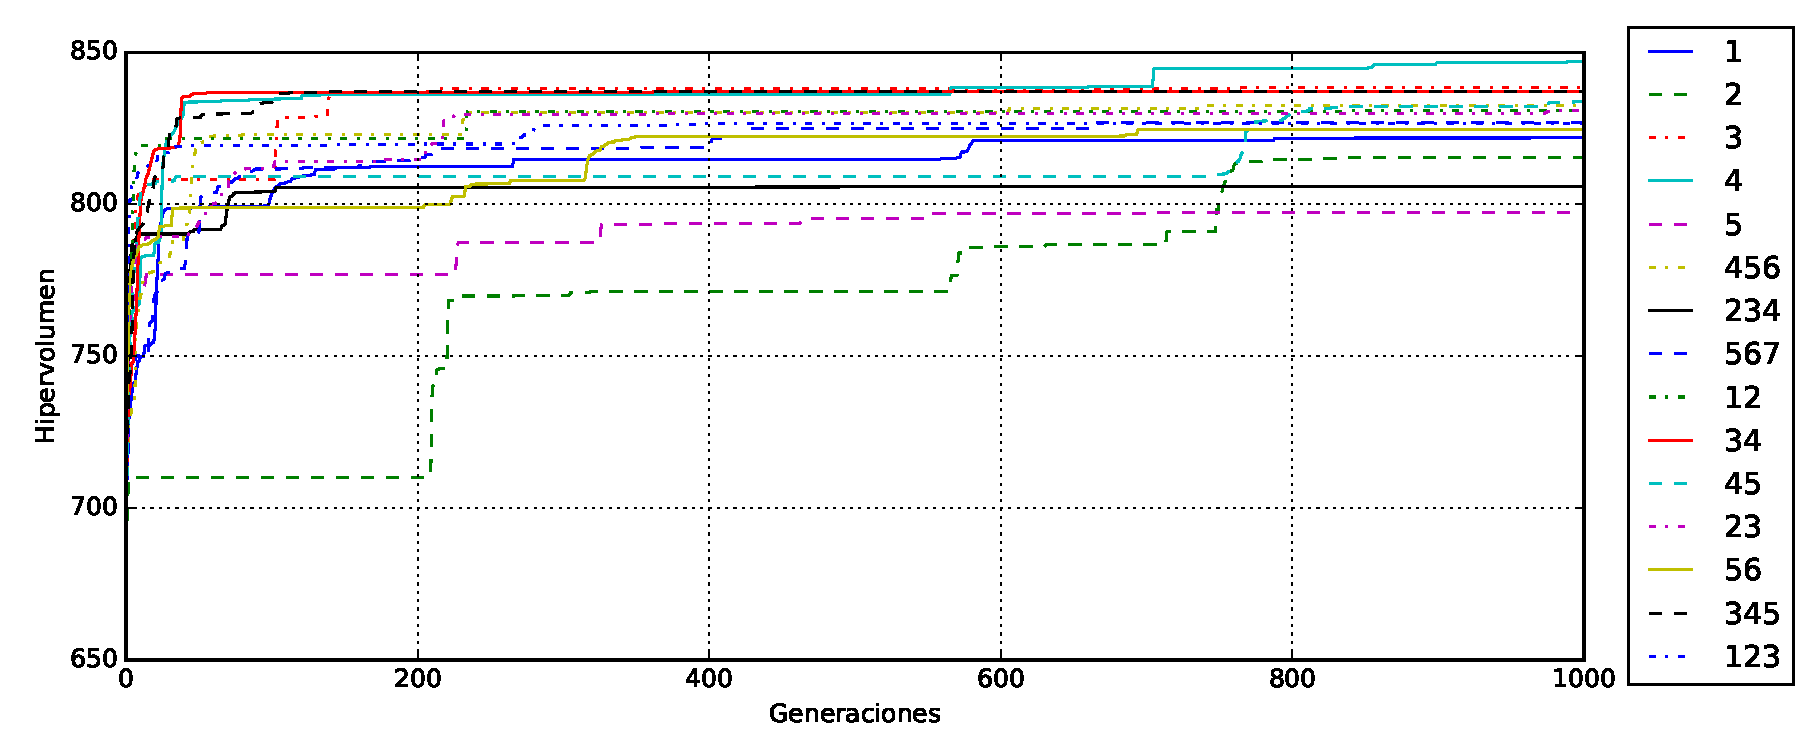
\includegraphics[width=\textwidth]{img/hyp_Mandl}
\caption{Hipervolumen obtenido en 15 semillas distintas con la instancia Mandl con sintonización de parámetros.}
\label{fig:hyp_mandl}
\end{figure}

\begin{figure}[!htb]
\centering
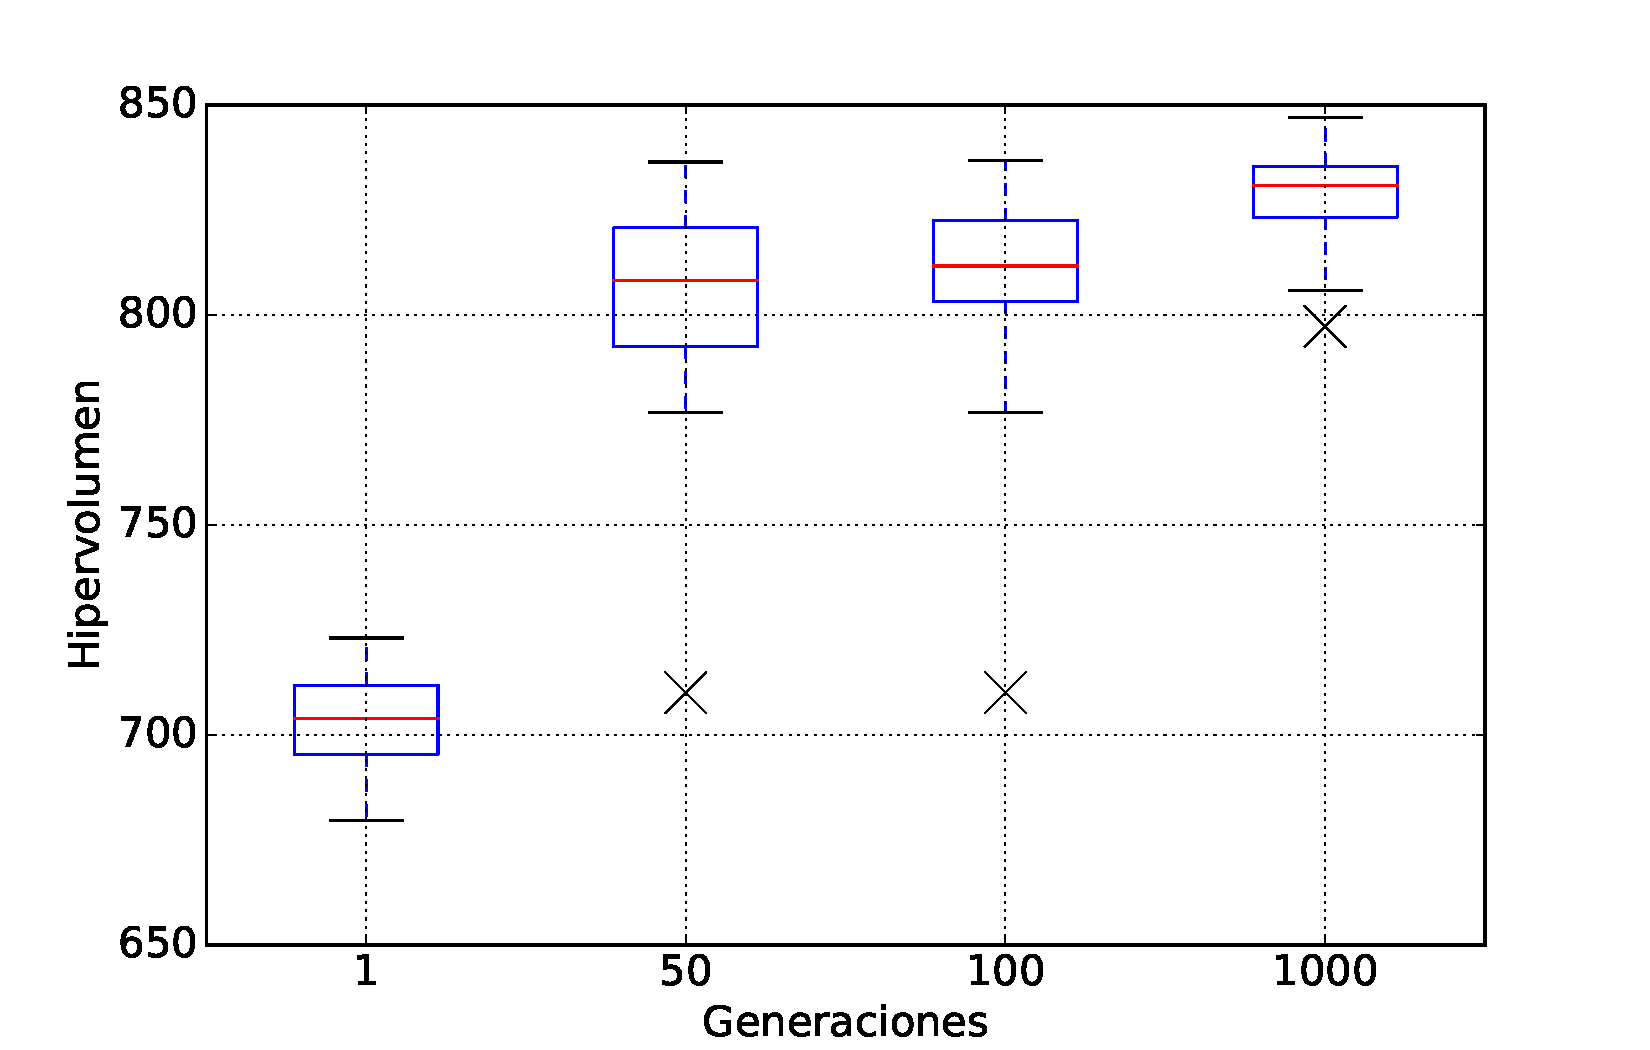
\includegraphics[width=\textwidth]{img/hyp_Mandl_bp}
\caption{Box plot del hipervolumen obtenido en distintas generaciones del algoritmo inmune para la instancia Mandl con sintonización de parámetros.}
\label{fig:hyp_mandl_bp}
\end{figure}

Al realizar experimentos para la instancia de Mandl con los mejores valores de los parámetros con 15 semillas distintas, se puede observar la variación de hipervolumen para todas ellas en la Figura \ref{fig:hyp_mandl}. Se observa que el comportamiento de la gráfica es el esperado para un algoritmo que va mejorando sus soluciones en cada generación. Se observa que en todos los casos hay periodos de estancamiento en las soluciones obtenidas, pero en ocasiones se produce una mejora súbita para pasar nuevamente a otro periodo de estancamiento. En general, a partir de la generación 200 no se observa una gran mejora en las soluciones obtenidas, ya que el hipervolumen se mantiene en niveles estables para cada caso. La Figura \ref{fig:hyp_mandl_bp} muestra la distibución de los valores del hipervolumen obtenidos con las 15 semillas en las generaciones 1, 50, 100 y 1000 del algoritmo para la instancia Mandl, utilizando los mejores valores de los parámetros para esta instancia. Se observa que a medida que aumentan las generaciones del algoritmo la mayoría de los valores se acerca a un valor de hipervolumen comprendido entre 800 y 850. Se puede decir entonces, que el algoritmo inmune propuesto no es afectado en gran medida por la aleatoridad introducida al utilizar distintas semillas en esta instancia.

A continuación, los frentes de Pareto resultantes de 4 semillas se pueden apreciar en las Figuras \ref{fig:paretoMandl1} y \ref{fig:paretoMandl2}. Además, información adicional de apoyo referente a estos frentes se encuentra en la Tabla \ref{tab:dataFrenteMandl}. En los casos mostrados, se observa que los frentes de Pareto se acercan a los mínimos de ambas funciones a medida que aumenta el número de generaciones. Adicionalmente, se puede ver la aparición de nuevas soluciones que no estaban definidas con anterioridad. El algoritmo propuesto es capaz de encontrar nuevas soluciones dentro de un vecindario de soluciones similares, producto de los operadores de mutación aplicados, los cual queda en evidencia con el aumento de soluciones del frente al aumentar el número de generaciones. Por otra parte, se obtienen mejoras en las soluciones ya encontradas, al visualizar el avance del frente de Pareto hacia el sector inferior izquierdo que tiene los mínimos de las dos funciones objetivo. Otro aspecto a notar en estas gráficas es la forma en que los frentes se van acercando al sector inferior izquierdo. Se observa claramente que el algoritmo propuesto obtiene muchas soluciones que son buenas para los pasajeros y pocas soluciones que son buenas para los operadores. 

\newpage

\begin{figure}[p]
\centering
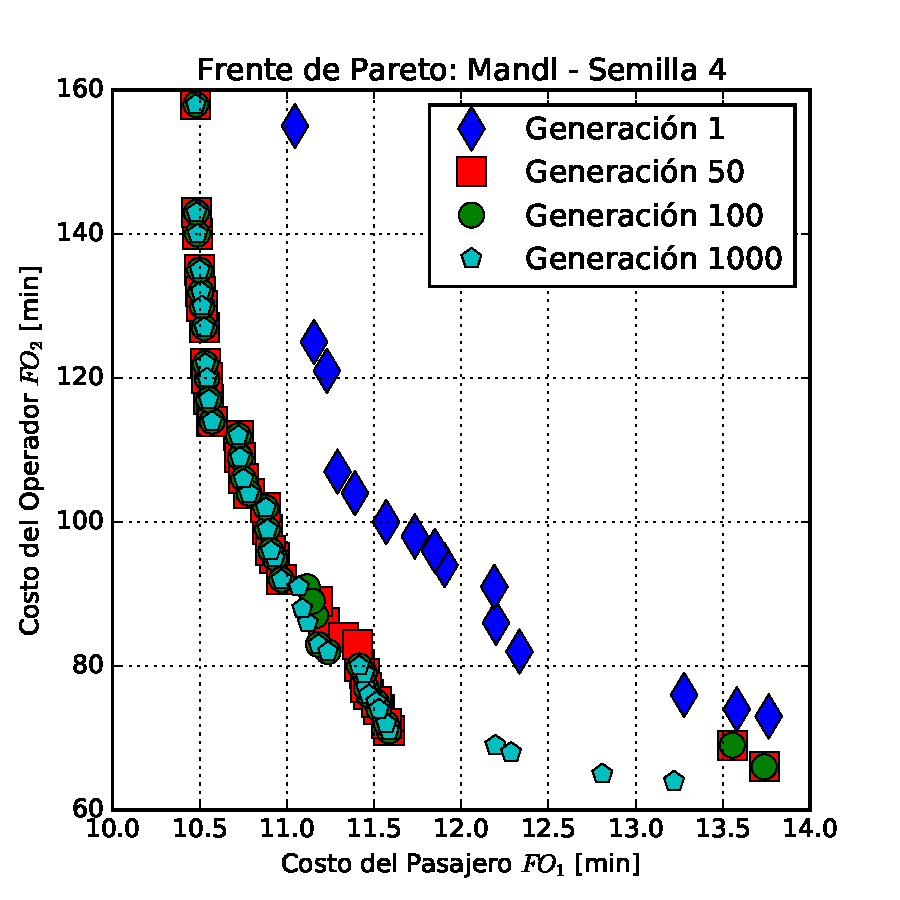
\includegraphics[width=0.79\textwidth]{img/frente_Mandl_s4}
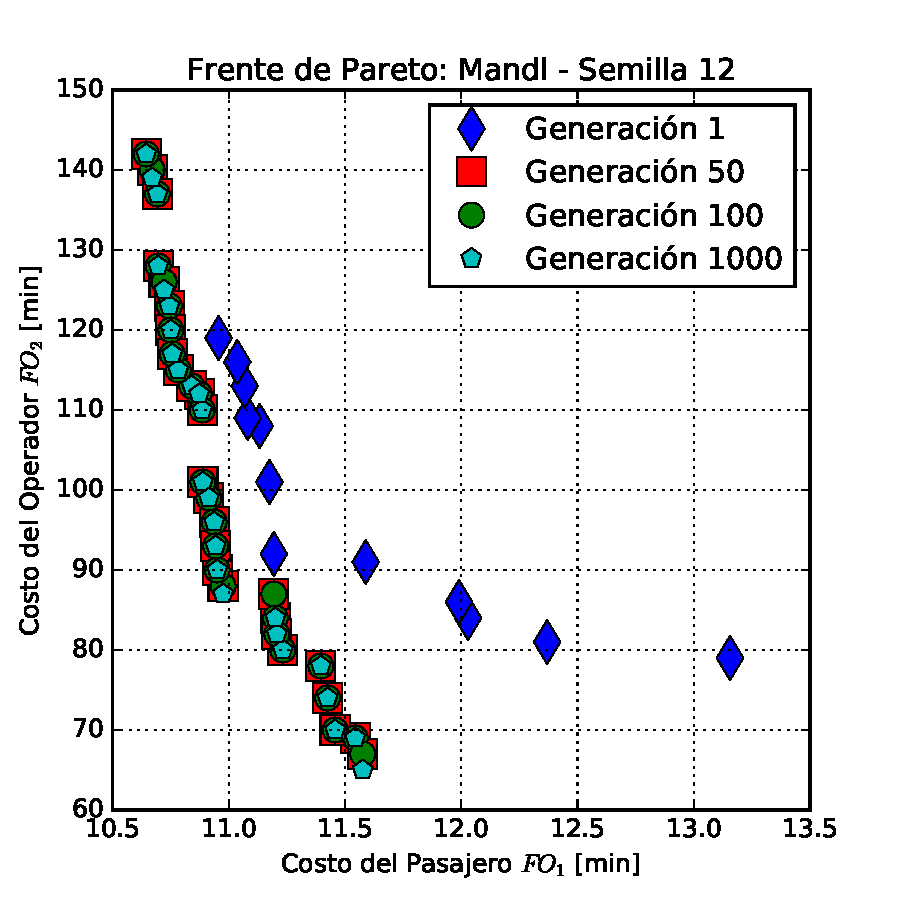
\includegraphics[width=0.79\textwidth]{img/frente_Mandl_s12}
\caption{Frente de Pareto para Mandl con semillas 4 y 12.}
\label{fig:paretoMandl1}
\end{figure}

\begin{figure}[p]
\centering
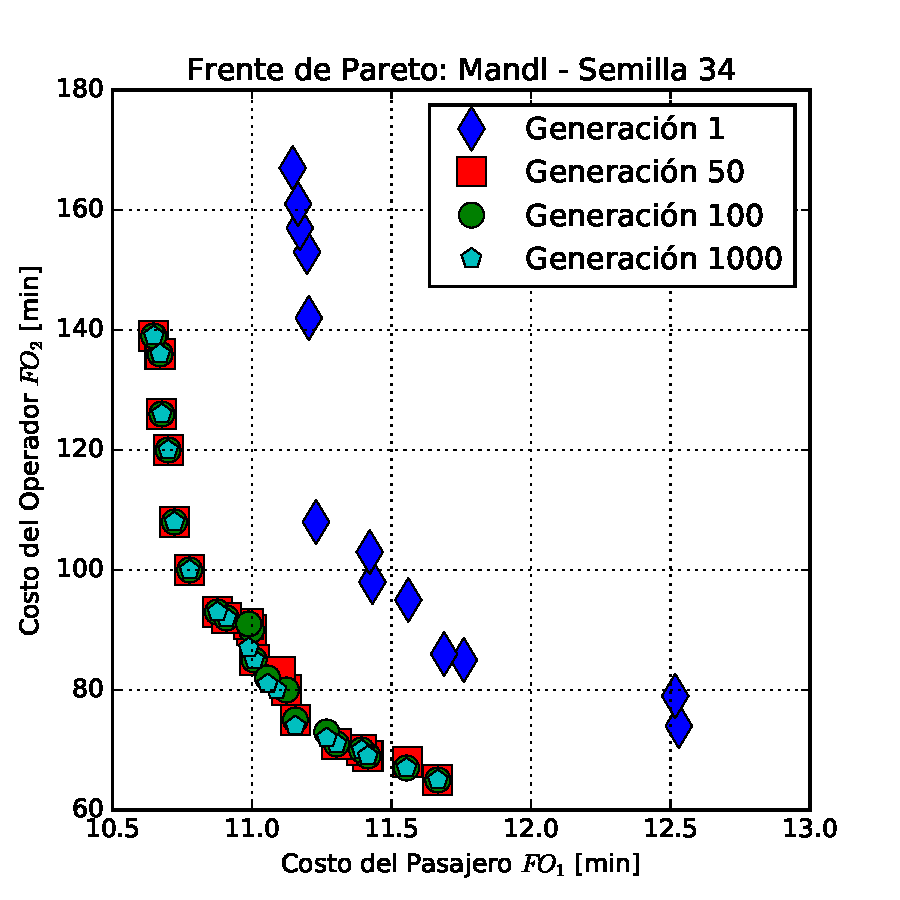
\includegraphics[width=0.79\textwidth]{img/frente_Mandl_s34}
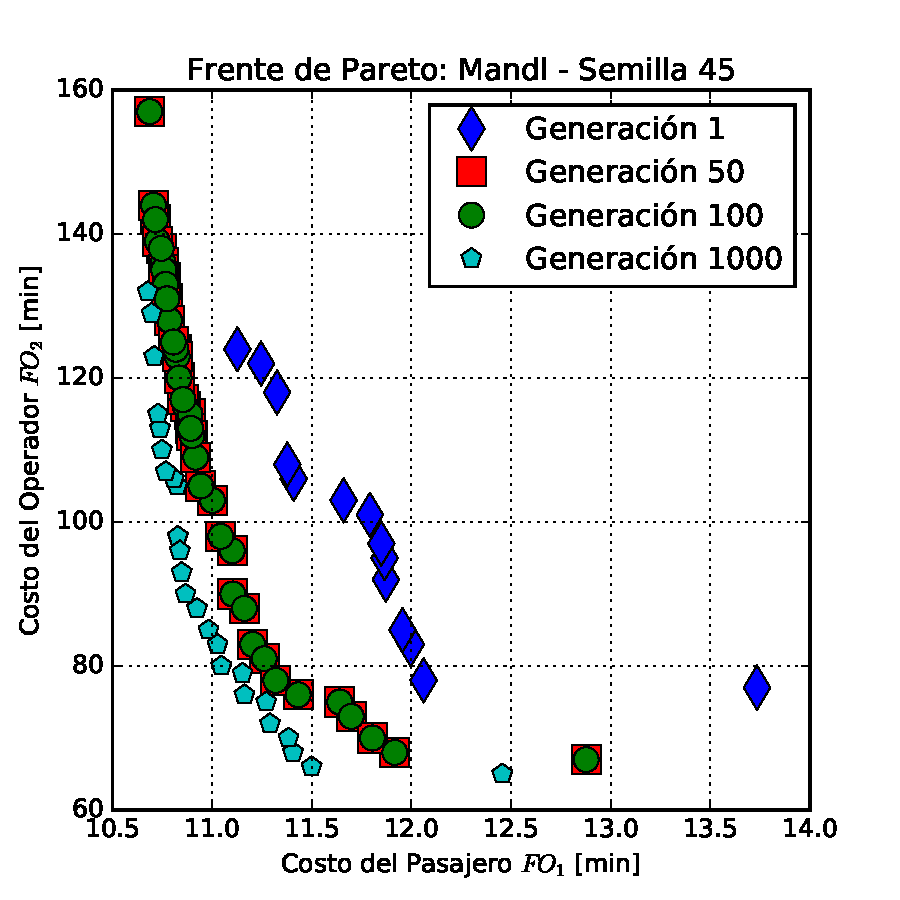
\includegraphics[width=0.79\textwidth]{img/frente_Mandl_s45}
\caption{Frente de Pareto para Mandl con semillas 34 y 45.}
\label{fig:paretoMandl2}
\end{figure}

\begin{table}[!htb]
\centering
\begin{tabular}{|r|r|r|r|r|r|}
\hline
Semilla & Generación & Sol. Únicas & Sol. Totales & Hipervolumen & Tiempo [s]\\ 
\hline \hline
4 & 1 & \textbf{15} & \textbf{15} & 702.207 & 26 \\ \hline
45 & 1 & 14 & 14 & 692.819 & 25 \\ \hline
12 & 1 & 12 & 12 & \textbf{714.867} & \textbf{22} \\ \hline
34 & 1 & 13 & 13 & 704.389 & \textbf{22} \\ \hline \hline
4 & 50 & 34 & 34 & 833.746 & 334 \\ \hline
45 & 50 & \textbf{36} & \textbf{36} & 809.110 & 344 \\ \hline
12 & 50 & 27 & 27 & 821.737 & 347 \\ \hline
34 & 50 & 19 & 19 & \textbf{836.426} & \textbf{325} \\ \hline\hline
4 & 100 & 35 & 65 & 834.683 & 645 \\ \hline
45 & 100 & \textbf{36} & \textbf{70} & 809.110 & 663 \\ \hline
12 & 100 & 27 & 27 & 821.737 & 683 \\ \hline
34 & 100 & 20 & 37 & \textbf{836.769} & \textbf{634} \\ \hline \hline
4 & 1000 & \textbf{37} & \textbf{335} & 847.025 & 6770 \\ \hline
45 & 1000 & 25 & 83 & 833.812 & 6533 \\ \hline
12 & 1000 & 26 & 153 & 830.848 & 6675 \\ \hline
34 & 1000 & 19 & 180 & \textbf{837.087} & \textbf{6357} \\ \hline
\end{tabular}
\caption{Cantidad de soluciones únicas/totales, hipervolumen y tiempo de cómputo en el frente de Pareto para 4 semillas de la instancia Mandl.}
\label{tab:dataFrenteMandl}
\end{table}

Por medio de la información de la Tabla \ref{tab:dataFrenteMandl} se destaca para este algoritmo en específico la aparición de muchas soluciones idénticas en los frentes de Pareto. Se puede observar, a modo general que desde la generación 50 y la generación 100 la soluciones totales son el doble de las soluciones únicas. En la generación 1000, las soluciones únicas representa entre un 10\% y un 30\% de las soluciones totales. En esta instancia se mantiene la tendencia de que la semilla que genera más soluciones únicas es la que tiene más soluciones totales. No existe una correlación entre un mayor hipervolumen con más soluciones únicas/totales en el frente. Finalmente, el tiempo para una instancia fue medido desde el inicio del algoritmo hasta la finalización de una generación. Tiempos menores en etapas prematuras del algoritmo suelen derivar en un tiempo total de cómputo menor para el algoritmo completo. Notar que al término de la generación 1 han transcurrido cerca de 20 segundos desde el inicio del algoritmo, donde este tiempo está destinado a la generación del conjunto inicial de soluciones factibles para iniciar el algoritmo.

En el caso de la instancia Mumford0, se realizó el mismo procedimiento, utilizando 15 semillas distintas con 1000 generaciones y los mejores valores  para los parámetros. La Figura \ref{fig:hyp_mumford0} muestra la evolución del hipervolumen para todas las semillas utilizadas y la Figura \ref{fig:hyp_mumford0_bp} muestra la distribución de los valores de hipervolumen para las semillas en las generaciones 1, 50, 100 y 1000 del algoritmo. En la Figura \ref{fig:hyp_mumford0} se observa que el hipervolumen aumenta su valor en todas las semillas utilizadas, notando estancamientos prolongados en este valor desde las 200 generaciones aproximadamente. En el \textit{box plot} de la Figura \ref{fig:hyp_mumford0_bp} se puede notar la aparición de \textit{outliers}. Sin embargo, para todas las semillas se observa el mismo comportamiento creciente, visto anteriormente. A modo general, el algoritmo no se ve afectado por la aleatoridad de una semilla determinada y tiende a obtener un valor de hipervolumen acotado.

\begin{figure}[!htb]
\centering
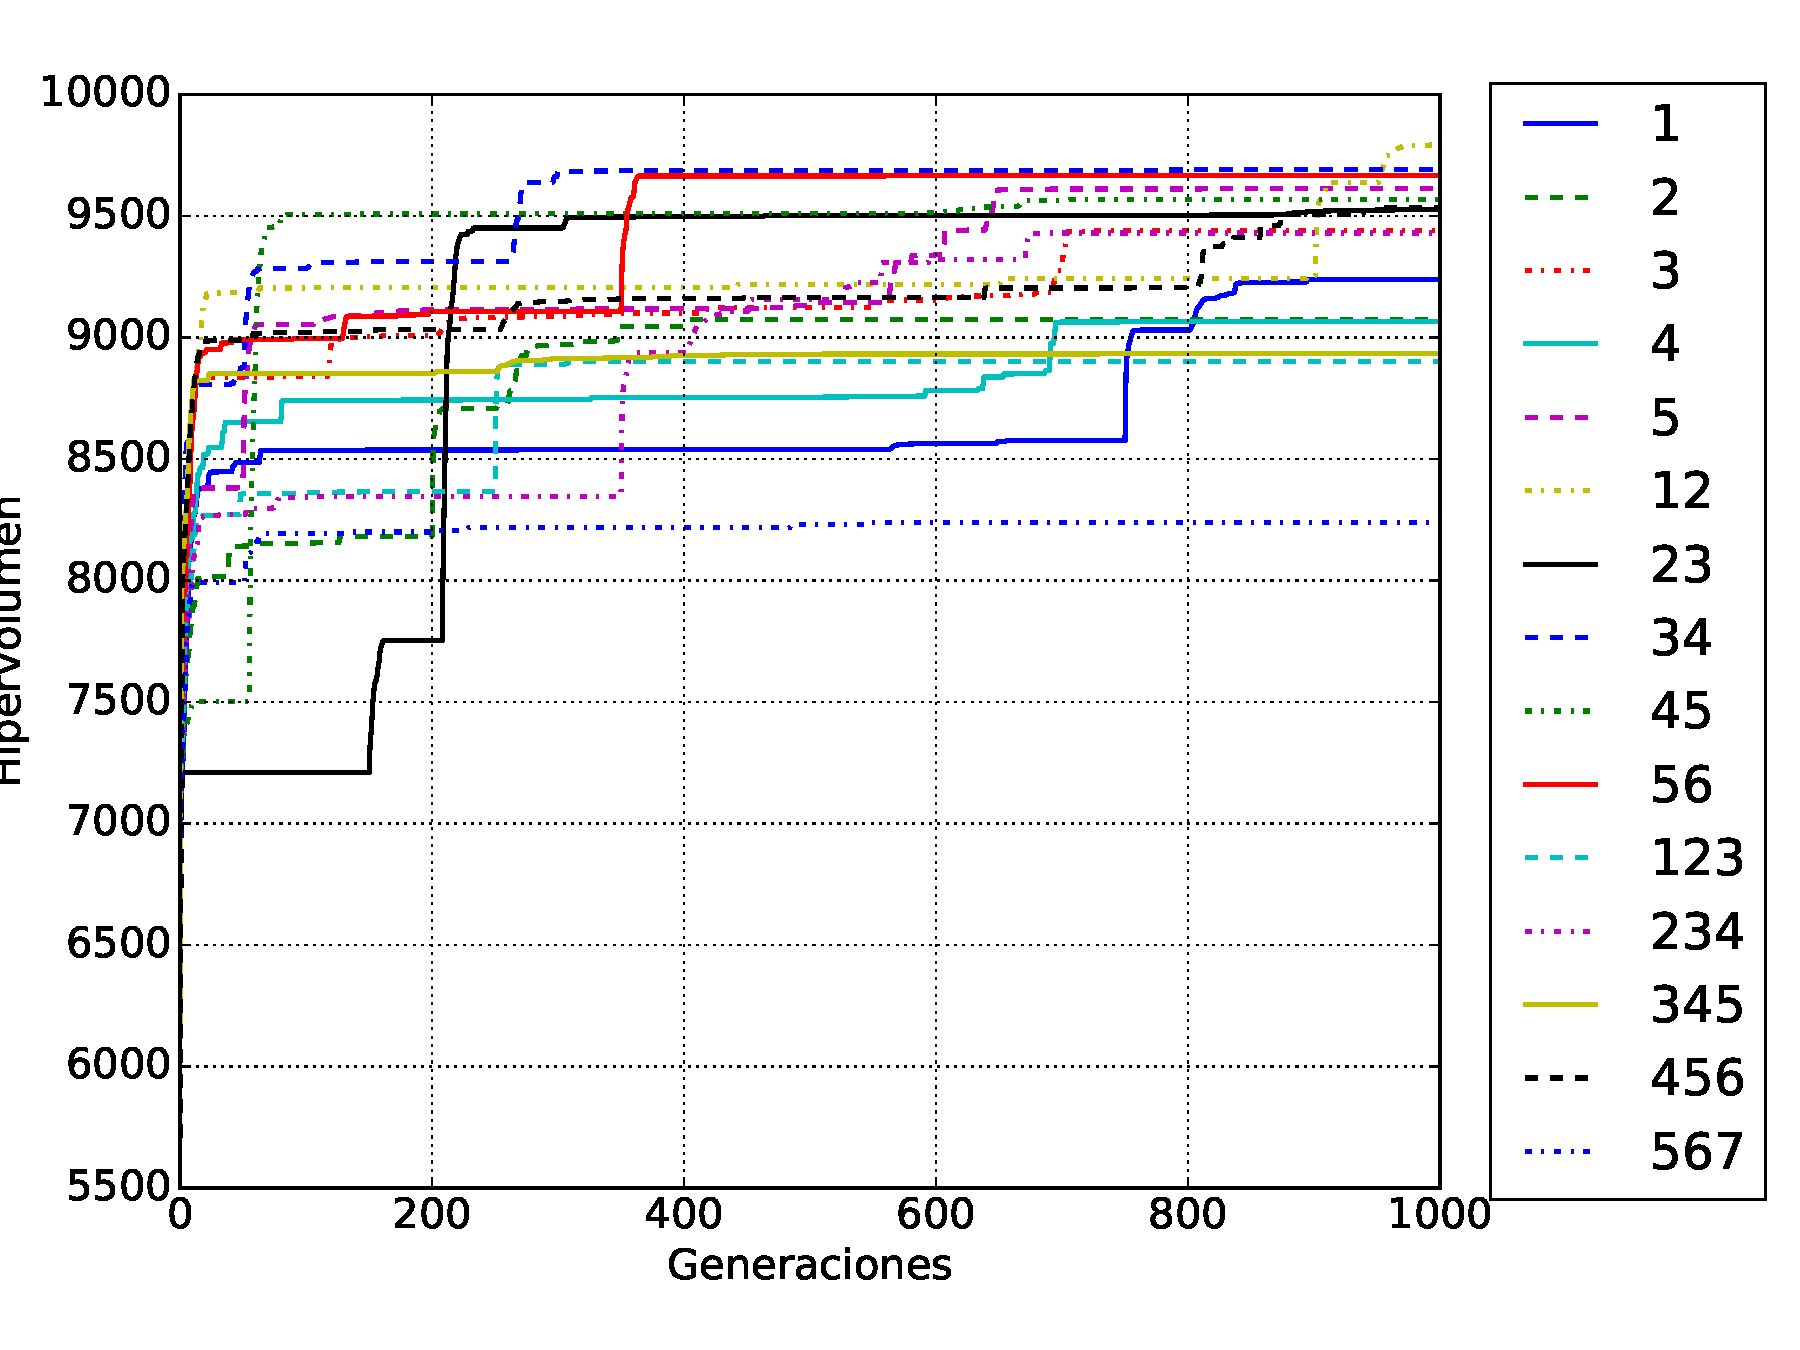
\includegraphics[width=\textwidth]{img/hyp_Mumford0}
\caption{Hipervolumen obtenido en 15 semillas distintas con la instancia Mumford0 con sintonización de parámetros.}
\label{fig:hyp_mumford0}
\end{figure}

\begin{figure}[!htb]
\centering
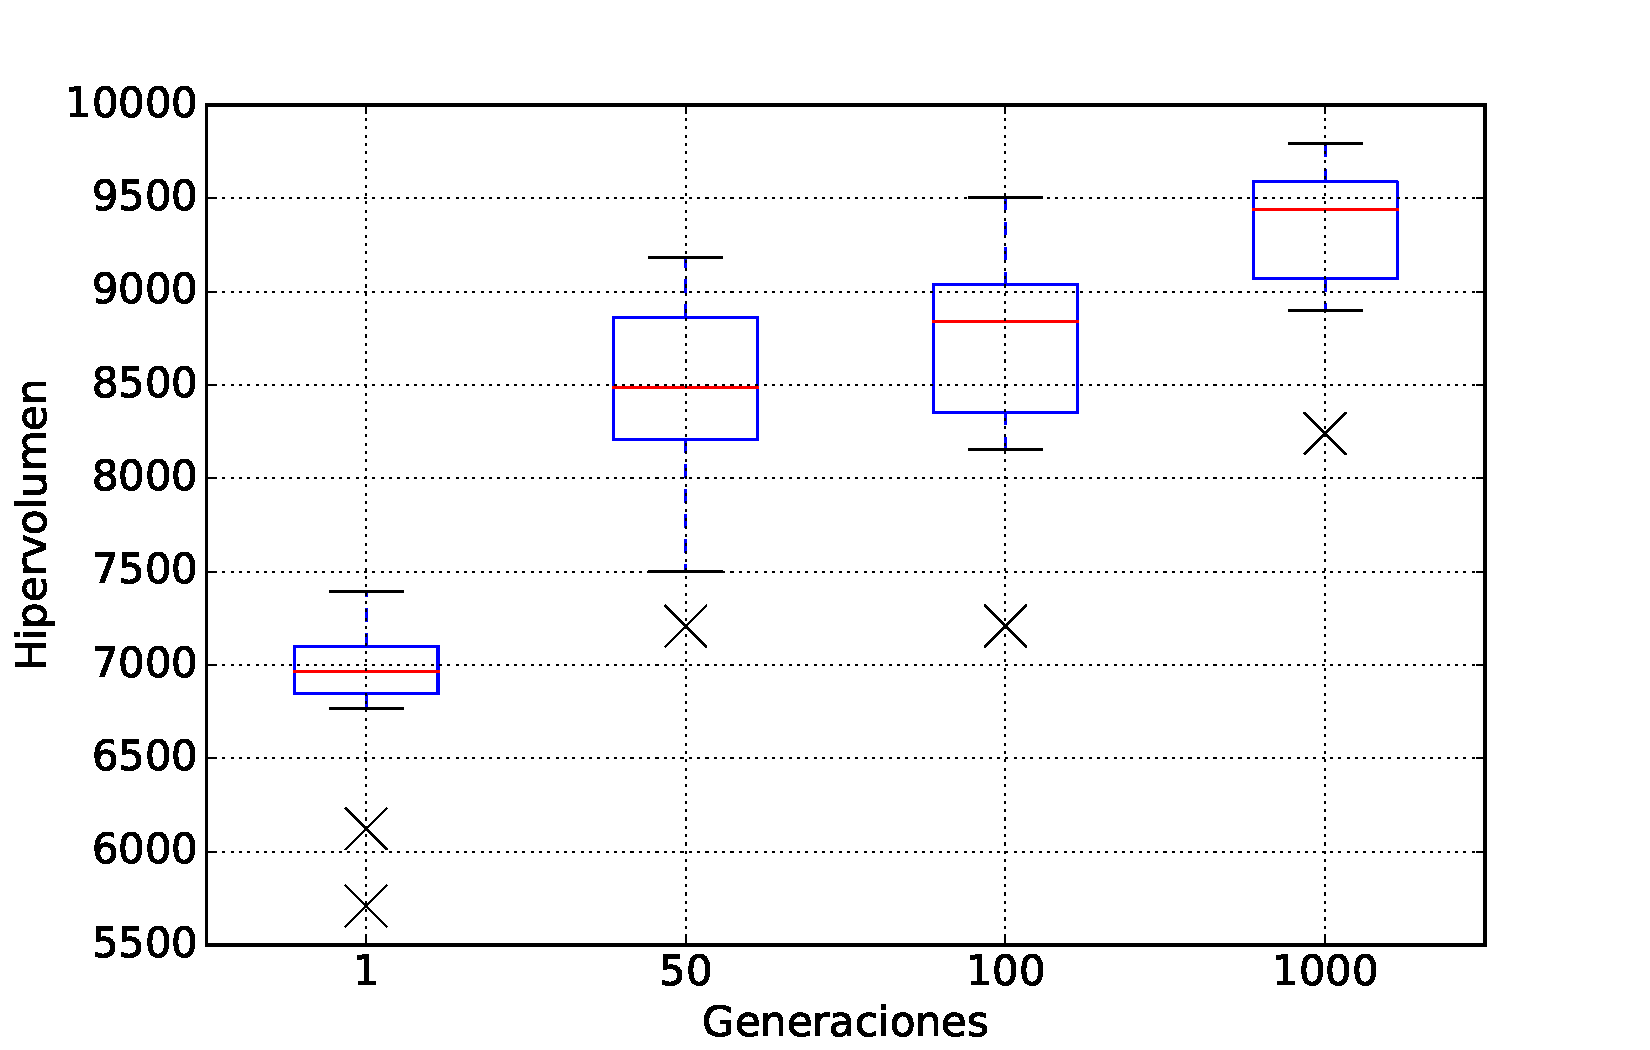
\includegraphics[width=\textwidth]{img/hyp_Mumford0_bp}
\caption{Box plot del hipervolumen obtenido en distintas generaciones del algoritmo inmune para la instancia Mumford0 con sintonización de parámetros.}
\label{fig:hyp_mumford0_bp}
\end{figure}

\begin{figure}[p]
\centering
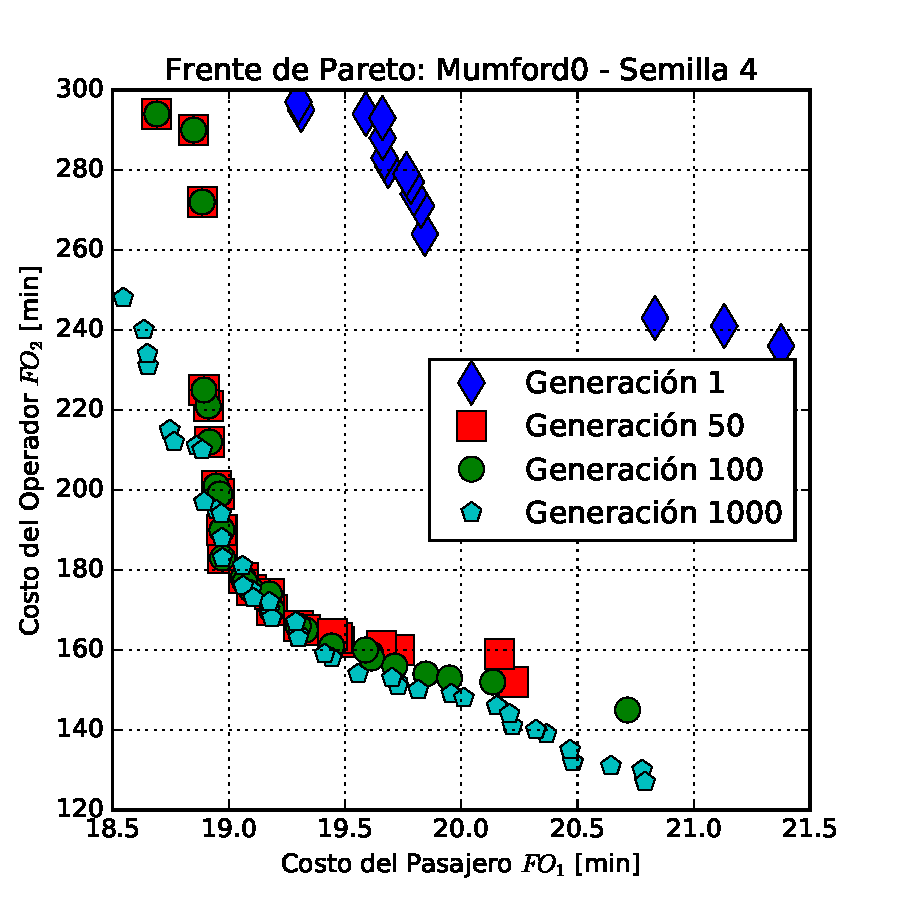
\includegraphics[width=0.79\textwidth]{img/frente_Mumford0_s4}
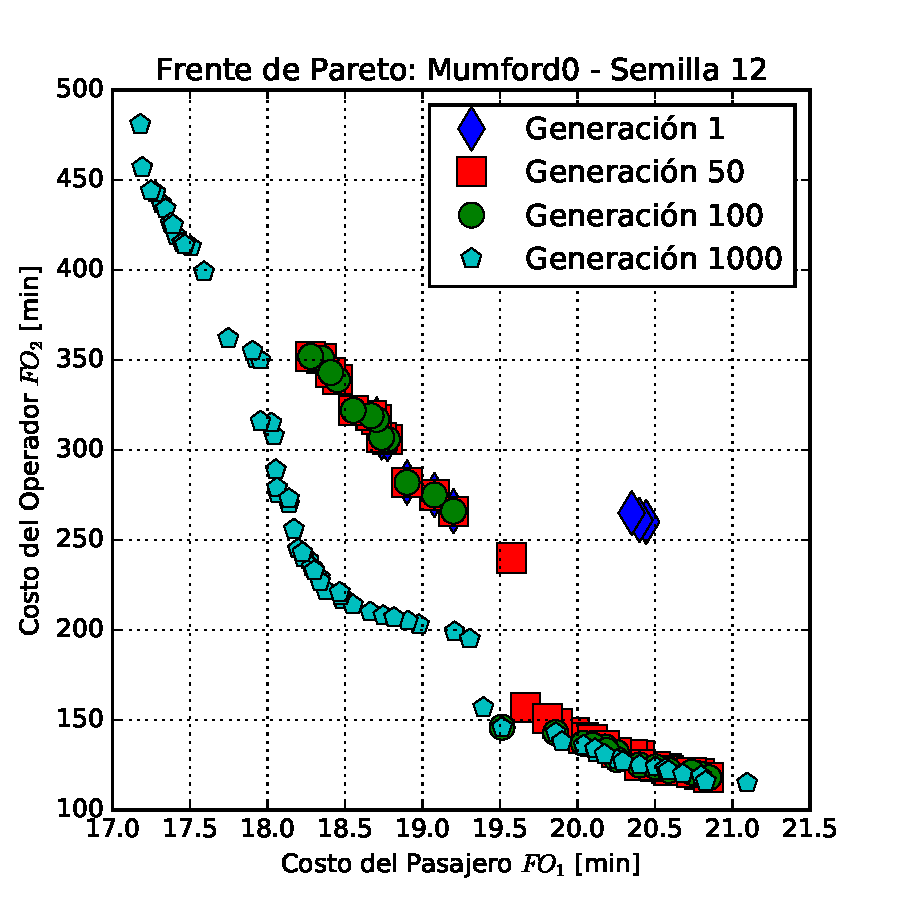
\includegraphics[width=0.79\textwidth]{img/frente_Mumford0_s12}
\caption{Frente de Pareto para Mumford0 con semillas 4 y 12.}
\label{fig:paretoMumford1}
\end{figure}

\begin{figure}[p]
\centering
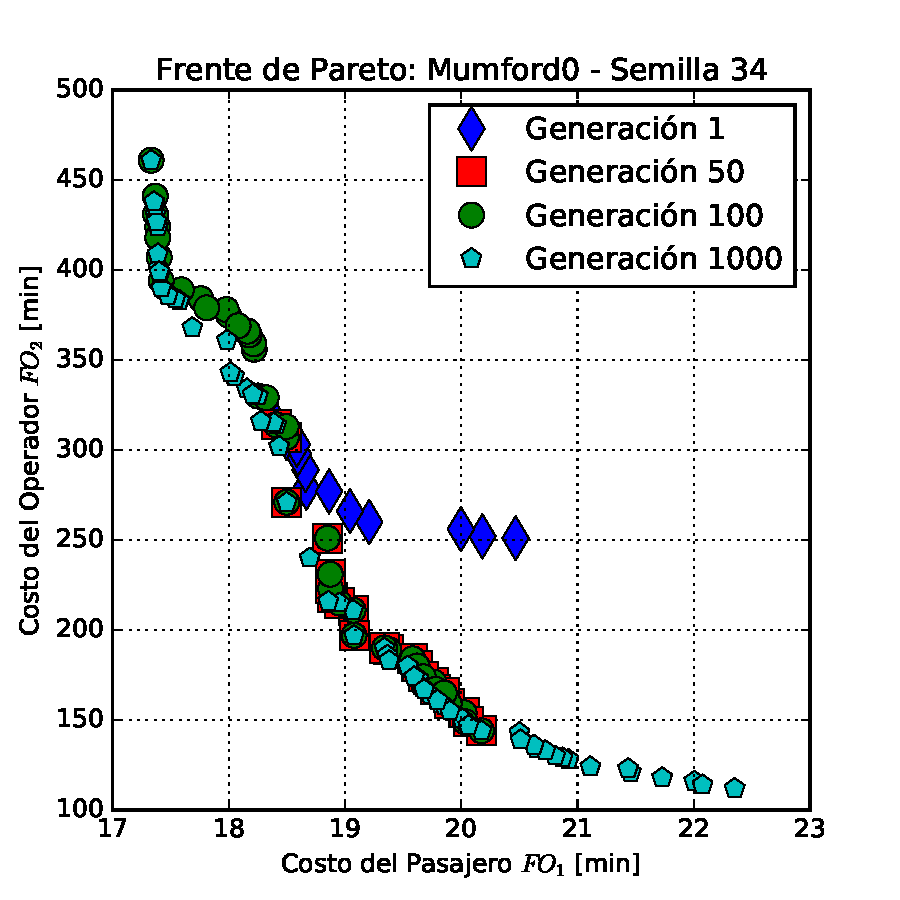
\includegraphics[width=0.79\textwidth]{img/frente_Mumford0_s34}
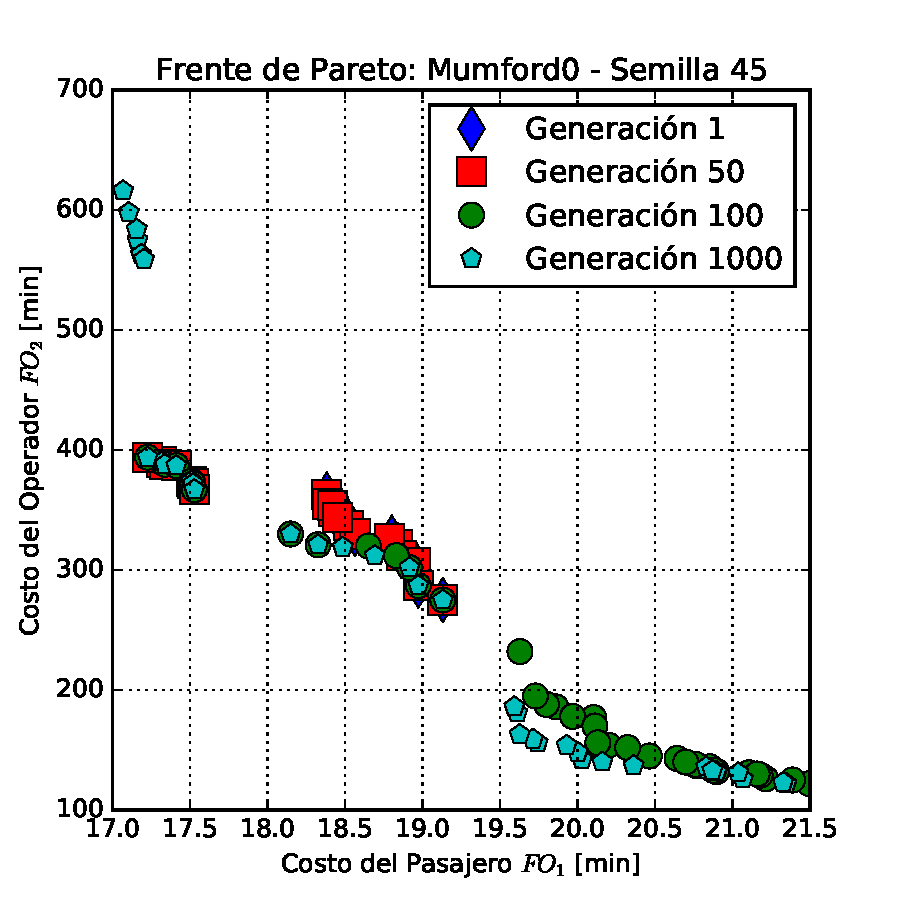
\includegraphics[width=0.79\textwidth]{img/frente_Mumford0_s45}
\caption{Frente de Pareto para Mumford0 con semillas 34 y 45.}
\label{fig:paretoMumford2}
\end{figure}

\begin{table}[!htb]
\centering
\begin{tabular}{|r|r|r|r|r|r|}
\hline
Semilla & Generación & Sol. Únicas & Sol. Totales & Hipervolumen & Tiempo [s]\\  
\hline \hline
4 & 1 & \textbf{15} & \textbf{15} & 7118.92 & \textbf{46} \\ \hline
45 & 1 & 12 & 12 & 7054.21 & 52 \\ \hline
12 & 1 & 9 & 9 & 7125.38 & 55 \\ \hline
34 & 1 & 12 & 12 & \textbf{7392.27} & 49 \\ \hline\hline
4 & 50 & 23 & 23 & 8650.36 & \textbf{1219} \\ \hline
45 & 50 & 20 & 20 & 7502.79 & 1742 \\ \hline
12 & 50 & \textbf{30} & \textbf{30} & \textbf{9185.21} & 1349 \\ \hline
34 & 50 & 22 & 22 & 8874.78 & 1276 \\ \hline\hline
4 & 100 & 26 & 33 & 8740.11 & \textbf{2280} \\ \hline
45 & 100 & 38 & 38 & \textbf{9506.56} & 3062 \\ \hline
12 & 100 & 27 & 30 & 9204.48 & 2622 \\ \hline
34 & 100 & \textbf{42} & \textbf{42} & 9285.58 & 3158 \\ \hline\hline
4 & 1000 & 42 & \textbf{103} & 9064.71 & \textbf{24308} \\ \hline
45 & 1000 & 38 & 38 & 9566.61 & 31216 \\ \hline
12 & 1000 & 64 & 85 & \textbf{9792.15} & 27600 \\ \hline
34 & 1000 & \textbf{65} & 83 & 9691.16 & 27324 \\ \hline\hline
\end{tabular}
\caption{Cantidad de soluciones únicas/totales, hipervolumen y tiempo de cómputo en el frente de Pareto para 4 semillas de la instancia Mumford0.}
\label{tab:dataFrenteMumford0}
\end{table}

Las Figuras \ref{fig:paretoMumford1} y \ref{fig:paretoMumford2} muestran la evolución del frente de Pareto en 4 semillas distintas y la Tabla \ref{tab:dataFrenteMumford0} muestra información adicional respecto a estos frentes. Se puede apreciar que la evolución del frente para semillas presenta un comportamiento favorable, ya que se acerca a la región de mínimos en ambas funciones objetivo. Un caso notable a mencionar ocurre con la semilla 4, donde se observa un gran avance a partir del frente inicial en la primera generación hasta el frente obtenido en la generación 50. A diferencia de la instancia Mandl, en estos casos se obtiene una buena cantidad de soluciones que son mejores para operadores y para pasajeros y el algoritmo tiene ciertas dificultades para acercarse a soluciones ubicadas en la zona inferior izquierda donde está el mínimo para operadores y pasajeros simultáneamente.

Al analizar los resultados de la Tabla \ref{tab:dataFrenteMandl} se puede observar que, en general, existe una repetición de soluciones candidatas que aumenta a medida que transcurren las generaciones. En esta instancia la cantidad de soluciones únicas representan una mayor parte de las soluciones totales que en la instancia Mandl. En las cuatro semillas mostradas, las soluciones únicas representan más del 40 \% de las soluciones totales en la milésima generación. En la semilla 45 en específico, la cantidad de soluciones únicas es igual a la cantidad de soluciones totales. Nuevamente, no es posible relacionar la cantidad de soluciones con el hipervolumen obtenido para una misma semilla en una generación determinada. Además, tampoco es posible afirmar que una semilla que inicia con un buen valor de hipervolumen, seguirá siendo la mejor semilla en la generación 1000. Los tiempos registrados al finalizar una generación dan cuenta de la misma relación que en Mandl, donde semillas que tardan menos tiempo en llegar a una generación tempranamente mantendrán la tendencia y demorarán menos tiempo en terminar con las 1000 generaciones. 

Las Tablas \ref{tab:mejoresfo1} y \ref{tab:mejoresfo2} muestran las mejores soluciones que se obtuvieron para las instancias Mandl y Mumford0, respectivamente. Es importante recordar que una solución corresponde a un conjunto de rutas acotado entre un mínimo y un máximo de paraderos, el cual debe satisfacer una serie de restriccciones. Los conjuntos de rutas que son mejores para 


\begin{table}[!htb]
\begin{center}
\begin{tabular}{|p{0.14\textwidth}|p{0.36\textwidth}|p{0.50\textwidth}|}
\hline
\multirow{2}{*}{Instancia} & \multicolumn{2}{c|}{Mejor solución para pasajeros (sintonización)} \\
\cline{2-3}
 & Costos & Rutas\\
\hline
\hline
Mandl & $C_p = 10.4778$\newline $C_o = 158$ \newline (semilla=4) & 9-15-6-3-2-1 \newline 3-2-5-4-6-8-10 \newline 4-2-3-6-15-7 \newline 11-10-8-6-3-2-1 \newline 9-15-7-10-11-12-4-2 \newline 11-13-14-10-7 \\
\hline
Mumford0 & $C_p = 17.0681$ \newline $C_o = 616$ \newline (semilla=45) & 8-29-17-3-16-22-7-14-1-13-9-20-18-12 \newline 24-15-2-5-4-10 \newline 27-1-26-12-15-8-3-7-6-16-11 \newline 2-5-25-8-3-30-28-16-22-11-7-6 \newline 18-1-14-7-6-22-3-16-30-28-8-5-2 \newline 27-9-13-20-23-18-1-19-14-7-3-28-17-8 \newline 7-3-11-17-16-28-8-21-15-10 \newline 7-14-19-1-26-23-18-12-4-2-5 \newline 21-8-26-1-13-9 \newline 4-2-5-8-3-7-14-19-13-23-1-20-18-12-15 \newline 30-3-22-6-16-7-14-1-20-18-29-17-28-11-8 \newline 28-11-22-6-7-17-16-3-8-25-2-4-5-15\\
\hline
\end{tabular}
\end{center}
\caption{Mejores soluciones para pasajeros por instancia.}
\label{tab:mejoresfo1}
\end{table}

\begin{table}[!htb]
\begin{center}
\begin{tabular}{|p{0.14\textwidth}|p{0.36\textwidth}|p{0.50\textwidth}|}
\hline
\multirow{2}{*}{Instancia} & \multicolumn{2}{c|}{Mejor solución para operadores (sintonización)}\\
\cline{2-3}
 & Costos & Rutas \\
\hline
\hline
Mandl & $C_p = 13.0501$\newline $C_o = 63$ \newline (semilla=567)  & 11-13-14 \newline 9-15-7 \newline 15-8-6-3-2-4-5 \newline 2-1 \newline 7-10 \newline 12-11-10 \\
\hline
Mumford0 & $C_p = 22.3516$ \newline $C_o = 112$ \newline (semilla=34) & 15-21 \newline 5-25-15 \newline 3-30-11-7 \newline 22-11 \newline 28-17-7-6 \newline 29-26-12 \newline 19-1 \newline 16-7-14 \newline 2-4-10-24 \newline 2-5-8-29-18-19-13-20-9-27 \newline 1-23 \newline 14-1 \\
\hline
\end{tabular}
\end{center}
\caption{Mejores soluciones para operadores por instancia.}
\label{tab:mejoresfo2}
\end{table}


\begin{table}[!htb]
\begin{center}
\begin{tabular}{|p{0.14\textwidth}|p{0.36\textwidth}|p{0.50\textwidth}|}
\hline
\multirow{2}{*}{Instancia} & \multicolumn{2}{c|}{Mejor solución para pasajeros (comparación)} \\
\cline{2-3}
 & Costos & Rutas\\
\hline
\hline
Mandl & $C_p = 10.5164$\newline $C_o = 149$ \newline (semilla=3) &  5-4-6-8-10-7-15-9 \newline  7-15-6-3-2-1 \newline  1-2 \newline  12-11-10-8-6-3-2-1 \newline  14-13-11-10-7 \newline  11-12-4-2-1\\
\hline
Mumford0 & $C_p = 17.3447$ \newline $C_o = 439$ \newline (semilla=2) &  28-30-11-17-29-8-26-12-15-25 \newline  4-2-25-5-8-11-22 \newline  19-18-1-29-8-17-7-11 \newline  8-25-4-12-18-19-14-7-6-16-3 \newline  5-25-2-10-15-24-21-8-3-7 \newline  13-23-19-18-20-9-27-1-26-8-5 \newline  8-21-24-25-5-4-15-2 \newline  26-23-20-1-14-19-18-13-9 \newline  24-21-5 \newline  11-7-14-1-13-9-20-18-12-4-2 \newline  3-22-7-16-11-8-28-17-29-1-13-9 \newline  3-17-29-1-13-9
\\
\hline
\end{tabular}
\end{center}
\caption{Mejores soluciones para pasajeros por instancia.}
\label{tab:mejoresfo1comp}
\end{table}


\begin{table}[!htb]
\begin{center}
\begin{tabular}{|p{0.14\textwidth}|p{0.36\textwidth}|p{0.50\textwidth}|}
\hline
\multirow{2}{*}{Instancia} & \multicolumn{2}{c|}{Mejor solución para operadores (comparación)} \\
\cline{2-3}
 & Costos & Rutas\\
\hline
\hline
Mandl & $C_p = 12.973$\newline $C_o = 63$ \newline (semilla=5678) & 6-3-2-1 \newline  2-4-5 \newline  12-11-10 \newline  11-13-14 \newline  9-15-7-10 \newline  15-8-6 \\
\hline
Mumford0 & $C_p = 21.4104$ \newline $C_o = 116$ \newline (semilla=1234) & 21-15 \newline  14-7-6 \newline  20-13-18-23-1-29 \newline  30-28-17 \newline  5-2-4-10 \newline  19-1 \newline  10-24-15-25 \newline  30-11-7 \newline  21-8-3 \newline  30-3 \newline  15-12-26-23-18-1-27-9 \newline  16-11-22 \\
\hline
\end{tabular}
\end{center}
\caption{Mejores soluciones para operadores por instancia.}
\label{tab:mejoresfo2comp}
\end{table}


%\section{Inicialización}

La inicialización del conjunto de soluciones inicial es determinado de manera aleatoria. De tal forma de tener contar con distintos lugares del espacio de búsqueda. Cada solución del conjunto contiene un conjunto de rutas, escogido de la siguiente manera: aleatoriamente se escoge un largo de ruta, el cual está comprendido entre el mínimo y máximo establecido. Se escoge aleatoriemente un punto de partida y se genera un camino mediante las conexiones con paradas vecinas hasta completar el largo. Se realiza este procedimiento hasta tener un conjunto de rutas que posea todos los paraderos disponibles o hasta que se agote un número de intentos, lo que puede ocurrir cuando el número de paraderos es muy grande en comparación con la cantidad de paraderos que serán destinados a una ruta o si el número de rutas a generar es muy pequeño. Las instancias con las que se trabajará siempre tratarán de incluír a todos los paraderos.\\

Se genera una población de soluciones de manera de tener varias soluciones candidatas. Este conjunto de soluciones inciales es un conjunto de soluciones factible, lo que quiere decir que las rutas generadas son conexas y además no presentan ciclos ni backtrackings. El algoritmo trabaja con soluciones factibles y al generar nuevas soluciones se comprueban las condiciones necesarias para que también sean factibles. 

\section{Proceso de transformación}

\subsection{Selección de soluciones}

El primer paso en el proceso de transformación del algoritmo consiste en realizar una selección clonal. Esto es, seleccionar a los mejores anticuerpos en base a una función de aptitud (\ref{eq:faptitud}). 

\begin{equation}
\label{eq:faptitud}
f_{aptitud}=\alpha \cdot FO_1 + \beta \cdot FO_2
\end{equation}

Donde $FO_1$ y $FO_2$ corresponden a las funciones objetivo dadas por las ecuaciones (\ref{eq:fo1}) y (\ref{eq:fo2}), respectivamente. Un porcentaje de estas soluciones son escogidas de acuerdo al resultado de $f_{aptitud}$ para pasar a la siguiente etapa del algoritmo.

\subsection{Operadores de transformación}

Los mejores anticuerpos son clonados hasta llegar a una cierta población. Esto consiste básicamente en generar muchas copias de los mejores anticuerpos. El operador de selección toma un anticuerpo y genera uno igual. La manera de decidir cual de los mejores anticuerpos se clona se realiza de manera aleatoria. De esta forma cada uno de los anticuerpos tiene la misma probabilidad de ser clonado.\\

Posteriormente, se utiliza un operador de mutación, el cual consiste en introducir pequeños cambios al conjunto de rutas para producir cambios en sus funciones objetivo, y por ende en la función de aptitud. La mutación consiste en seleccionar aleatoriamente una ruta de una solucion e introducir un nuevo vertice en ella, siempre y cuando no exceda el límite superior.


\subsection{Selección de soluciones para conformar nueva población}

Luego, se aplica una reducción de la población de los clones, dejando los más aptos (con una mejor función de aptitud). Se procede a reemplazar a los peores anticuerpos con anticuerpos generados aleatoriamente, siguiendo las mismas restricciones de la generación inicial al generar soluciones candidatas factibles. 



\section{Sintonización de Parámetros}

Para la sintonización de parámetros se escogieron 4 de los parámetros y el resto quedó con un valor fijo. Entre los parámetros con valor fijo se utilizaron los valores de la Tabla \ref{tab:paramfijos}. La instancia utilizada fue la de \texttt{Mandl 6:2:8}, cuyo grafo está representado en la Figura \ref{fig:mandl}. Se buscan 6 rutas con longitudes que varían en el rango de 2 a 8 paradas.

\begin{table}[!htb]
\begin{center}
\begin{tabular}{|c|c|}
\hline
\texttt{ALPHA} & 1.0\\ \hline
\texttt{BETA} & 1.0\\ \hline
\texttt{AFINIDAD} & 1\\ \hline
\texttt{REEMPLAZO} & 0.01\\ \hline
\end{tabular}
\label{tab:paramfijos}
\caption{Parámetros seteados en un valor fijo para Mandl.}
\end{center}
\end{table}

Los parámetros \texttt{POP\_SIZE}, \texttt{CLON\_SIZE}, \texttt{GENERACIONES} y \texttt{CLONES} fueron puestos a prueba al utilizar ParamILS, un sintonizador de parámetros que utiliza un intérprete del código y ejecuta el algoritmo utilizando un rango de valores para los 4 parámetros escogidos.

\begin{figure}[!htb]
\begin{verbatim}
ps {20, 40, 100, 160, 200}[100]
cs {5, 15, 25}[15]
it {10, 30, 50, 70, 100}[30]
pc {10, 30, 50}[10]
\end{verbatim}
\caption{Valores utilizados en los parámetros sintonizados en Mandl.}
\label{fig:paramsintonizados}
\end{figure}

En la Figura \ref{fig:paramsintonizados} \texttt{ps}, \texttt{cs}, \texttt{it} y \texttt{pc} corresponden a \texttt{POP\_SIZE}, \texttt{CLON\_SIZE}, \texttt{GENERACIONES} y \texttt{CLONES} respectivamente.

\newpage

Al ejecutar ParamILS se obtuvo la siguiente salida:

\begin{small}
\begin{verbatim}
Final best parameter configuration: cs=5, it=100, pc=10, ps=200
==================================================================
Active parameters: cs=5, it=100, pc=10, ps=200
==================================================================
Training quality of this final best found parameter configuration: 
-704.619631901841, based on 163 runs with cutoff 1000000000.0
Test quality of this final best found parameter configuration: 
-703.96, based on 50 independent runs with cutoff 1000000000.0
\end{verbatim}
\end{small}

Para este valores de parámetros se obtuvo un valor máximo de hipervolumen igual a 703.96.

\section{Experimentos}

El experimento con los valores de parámetros fijados según la Tabla \ref{tab:paramfijos} y los obtenidos mediante ParamILS, según lo mostroado a continuación:

\begin{table}[!htb]
\begin{center}
\begin{tabular}{|c|c|}
\hline
POP SIZE & 200\\ \hline
ALPHA & 1.0\\ \hline
BETA & 1.0\\ \hline
CLON SIZE & 5\\ \hline
AFINIDAD & 1\\ \hline
GENERACIONES & 100\\ \hline
CLONES & 0.1\\ \hline
REEMPLAZO & 0.01\\ \hline
\end{tabular}
\caption{Valores utilizados para el experimento con la instancia de Mandl.}
\end{center}
\end{table}

Notar que el porcentaje de clones fue manejado en ParamILS con valores entre 0 y 100 y pasado posteriormente a valores entre 0 y 1.

\begin{figure}[!htb]
\begin{center}
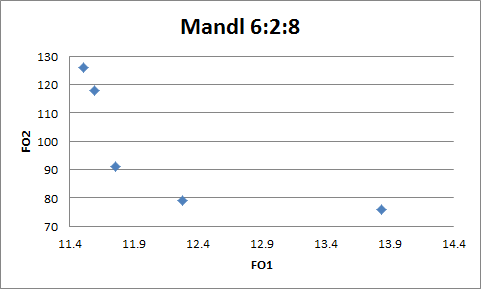
\includegraphics[scale=0.7]{pareto_mandl.png}
\caption{Frente de Pareto de la instancia de Mandl.}
\label{fig:pareto_mandl}
\end{center}
\end{figure}

\begin{table}[!htb]
\begin{center}
\begin{tabular}{|l|c|}
\hline
Hipervolumen & 698.452\\ \hline
Tiempo de ejecución & 23 segundos\\ \hline
\end{tabular}
\caption{Hipervolumen y tiempo de ejecución.}
\label{tab:mandldata}
\end{center}
\end{table}

Además, los mejores valores para las funciones objetivo corresponden a:
\begin{itemize}
\item Mejor FO1: 11.5087
\item Mejor FO2: 76
\end{itemize}

\newpage
El conjunto de rutas que presenta el menor valor para la función de aptitud se muestra a continuación:
\begin{verbatim}
6-3
9-15-6-8
3-2-4-12
8-6-3
8-15-7-10-14-13-11
1-2-5
\end{verbatim}

Se puede concluir que estos resultados no reflejan exactamente a lo obtenido mediante la sintonización de parámetros porque esto corresponde solo a una ejecución del algoritmo. Por otra parte, ParamILS realiza una cantidad considerable de experimentos probando con distintos valores y logra encontrar el mejor valor de hipervolumen. En este caso el valor es cercano al mejor valor obtenido, sin embargo si se realizara otro experimento podría originar un valor más cercano o más lejano.

\section{Conclusiones}

Los algoritmos inmunes artificiales utilizan analogías de los organismos vivos. Cuando un virus ataca al organismo los anticuerpos son capaces de interactuar con este y los más capaces son duplicados para atacar y eliminar a una enfermedad que cause. Luego se guarda en memoria una cantidad menor de este anticuerpo para que esté preparado a nuevas infecciones del mismo virus o uno similar. Esta idea es la que permite encontrar soluciones mediante la clonación y mutación de los mejores individuos. El proceso de búsqueda de soluciones es un proceso adaptativo, lo que quiere decir que los anticuerpos se capacitan para enfrentarse a infecciones futuras. \\

Mediante esta implementación, la cual está compuesta por variables, restricciones, funciones objetivo, función de aptitud, operadores de selección y transformación para una población de anticuerpos se pudo encontrar un conjunto de soluciones no dominadas según Pareto, obteniendo mejores soluciones en tiempos relativamente cortos. \\

El proceso de sintonización de parámetros fue útil para poder encontrar valores para parámetros y obtener un mejor resultado, el cual está reflejado en un mayor valor de hipervolumen.\\



\section{Bibliograf\'ia}
\bibliographystyle{plain}
\bibliography{utrp}

\end{document}
